% F049: native TikZ/PGFPlots, computed from the stated mathematical model.
\begin{center}
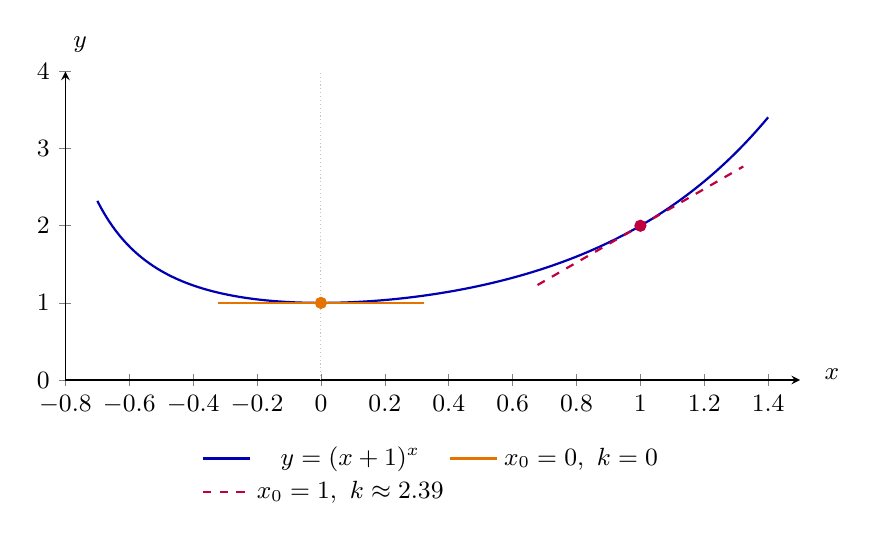
\begin{tikzpicture}[font=\small,>=stealth]
\begin{axis}[width=.90\linewidth,height=5.5cm,xmin=-0.8,xmax=1.5,ymin=0,ymax=4,
axis lines=left,xlabel={$x$},ylabel={$y$},font=\small,
xlabel style={at={(axis description cs:1.02,.02)},anchor=west},
ylabel style={rotate=-90,at={(axis description cs:.02,1.03)},anchor=south},
legend style={at={(axis description cs:.5,-.18)},anchor=north,draw=none,fill=none,font=\small,legend columns=2},
unbounded coords=jump,clip=true,]
\addplot[gray!45,thin,densely dotted,forget plot] coordinates {(0,0) (0,4)};
\addplot[blue!70!black,thick] coordinates {(-0.7,2.3228177) (-0.68833333,2.2310526) (-0.67666667,2.1468573) (-0.665,2.0694036) (-0.65333333,1.9979783) (-0.64166667,1.931964) (-0.63,1.8708239) (-0.61833333,1.814089) (-0.60666667,1.7613479) (-0.595,1.7122385) (-0.58333333,1.6664408) (-0.57166667,1.623671) (-0.56,1.5836766) (-0.54833333,1.5462324) (-0.53666667,1.5111369) (-0.525,1.478209) (-0.51333333,1.4472863) (-0.50166667,1.4182218) (-0.49,1.390883) (-0.47833333,1.3651498) (-0.46666667,1.340913) (-0.455,1.3180734) (-0.44333333,1.2965406) (-0.43166667,1.2762321) (-0.42,1.2570723) (-0.40833333,1.238992) (-0.39666667,1.2219279) (-0.385,1.2058217) (-0.37333333,1.1906195) (-0.36166667,1.1762721) (-0.35,1.1627339) (-0.33833333,1.1499626) (-0.32666667,1.1379194) (-0.315,1.1265682) (-0.30333333,1.1158755) (-0.29166667,1.1058104) (-0.28,1.0963441) (-0.26833333,1.0874499) (-0.25666667,1.0791029) (-0.245,1.07128) (-0.23333333,1.0639596) (-0.22166667,1.0571216) (-0.21,1.0507474) (-0.19833333,1.0448194) (-0.18666667,1.0393214) (-0.175,1.0342382) (-0.16333333,1.0295555) (-0.15166667,1.0252601) (-0.14,1.0213397) (-0.12833333,1.0177826) (-0.11666667,1.014578) (-0.105,1.0117159) (-0.093333333,1.0091868) (-0.081666667,1.0069818) (-0.07,1.0050929) (-0.058333333,1.0035122) (-0.046666667,1.0022327) (-0.035,1.0012477) (-0.023333333,1.000551) (-0.011666667,1.0001369) (-1.110223e-16,1) (0.011666667,1.0001353) (0.023333333,1.0005383) (0.035,1.0012048) (0.046666667,1.0021308) (0.058333333,1.0033127) (0.07,1.0047473) (0.081666667,1.0064317) (0.093333333,1.008363) (0.105,1.0105389) (0.11666667,1.0129572) (0.12833333,1.0156158) (0.14,1.0185132) (0.15166667,1.0216479) (0.16333333,1.0250184) (0.175,1.0286239) (0.18666667,1.0324635) (0.19833333,1.0365364) (0.21,1.0408423) (0.22166667,1.0453808) (0.23333333,1.0501519) (0.245,1.0551556) (0.25666667,1.0603921) (0.26833333,1.065862) (0.28,1.0715657) (0.29166667,1.077504) (0.30333333,1.0836778) (0.315,1.0900881) (0.32666667,1.0967362) (0.33833333,1.1036234) (0.35,1.1107513) (0.36166667,1.1181214) (0.37333333,1.1257355) (0.385,1.1335956) (0.39666667,1.1417038) (0.40833333,1.1500624) (0.42,1.1586736) (0.43166667,1.16754) (0.44333333,1.1766642) (0.455,1.1860491) (0.46666667,1.1956975) (0.47833333,1.2056126) (0.49,1.2157976) (0.50166667,1.2262558) (0.51333333,1.2369907) (0.525,1.248006) (0.53666667,1.2593055) (0.54833333,1.2708931) (0.56,1.2827729) (0.57166667,1.2949492) (0.58333333,1.3074263) (0.595,1.3202088) (0.60666667,1.3333013) (0.61833333,1.3467088) (0.63,1.3604362) (0.64166667,1.3744888) (0.65333333,1.3888717) (0.665,1.4035907) (0.67666667,1.4186512) (0.68833333,1.4340591) (0.7,1.4498205) (0.71166667,1.4659416) (0.72333333,1.4824286) (0.735,1.4992882) (0.74666667,1.516527) (0.75833333,1.5341521) (0.77,1.5521705) (0.78166667,1.5705895) (0.79333333,1.5894166) (0.805,1.6086596) (0.81666667,1.6283264) (0.82833333,1.648425) (0.84,1.668964) (0.85166667,1.6899518) (0.86333333,1.7113973) (0.875,1.7333095) (0.88666667,1.7556976) (0.89833333,1.7785713) (0.91,1.8019402) (0.92166667,1.8258143) (0.93333333,1.850204) (0.945,1.8751198) (0.95666667,1.9005725) (0.96833333,1.9265732) (0.98,1.9531333) (0.99166667,1.9802644) (1.0033333,2.0079785) (1.015,2.0362879) (1.0266667,2.0652051) (1.0383333,2.094743) (1.05,2.124915) (1.0616667,2.1557344) (1.0733333,2.1872153) (1.085,2.2193719) (1.0966667,2.2522187) (1.1083333,2.2857709) (1.12,2.3200437) (1.1316667,2.3550529) (1.1433333,2.3908147) (1.155,2.4273455) (1.1666667,2.4646625) (1.1783333,2.5027829) (1.19,2.5417246) (1.2016667,2.581506) (1.2133333,2.6221457) (1.225,2.6636629) (1.2366667,2.7060775) (1.2483333,2.7494096) (1.26,2.7936798) (1.2716667,2.8389096) (1.2833333,2.8851205) (1.295,2.932335) (1.3066667,2.9805759) (1.3183333,3.0298668) (1.33,3.0802316) (1.3416667,3.1316951) (1.3533333,3.1842826) (1.365,3.2380199) (1.3766667,3.2929337) (1.3883333,3.3490514) (1.4,3.4064007)};
\addlegendentry{$y=(x+1)^x$}
\addplot[orange!90!black,thick] coordinates {(-0.322,1) (0.322,1)};
\addlegendentry{$x_0=0,\ k=0$}
\addplot[only marks,mark=*,orange!90!black,forget plot] coordinates {(0,1)};
\addplot[purple,thick,dashed] coordinates {(0.678,1.2316132) (1.322,2.7683868)};
\addlegendentry{$x_0=1,\ k\approx2.39$}
\addplot[only marks,mark=*,purple,forget plot] coordinates {(1,2)};

\end{axis}
\end{tikzpicture}
\par\smallskip{\small 推广公式的实例：$u=x+1>0,v=x$，$y\prime=(x+1)^x[\ln(x+1)+x/(x+1)]$。}
\end{center}
